% Provenance (never printed): cycle 4 SVT, "La planete Terre, l'environnement
% et l'action humaine": climate, its past variations and the present change,
% read from data; see sources/book1/PROVENANCE.md. Book 1, grade 9, chapter 1.
% Vocabulary guard: owns climate change (first look; Book 2 g12 re-uses it),
% global warming, temperature anomaly. The greenhouse effect and greenhouse
% gases belong to the chemistry series (grade 8): recalled in prose, never
% defined. Infrared is physics (g10): named in prose only. "Glacial period"
% and "interglacial" belong to Book 2 g12: here "the ice ages and the warmer
% times between them". Physical science only, in the IPCC's calibrated words;
% no policy.
\chapter{The Earth's Climate, Past and Present}\label{ch:g9:climate-past-and-present}

If the Earth had no air around it, but reflected the same share of
sunlight as it does today, its surface would settle at an average
temperature of about \qty{-19}{\degreeCelsius}: frozen \omterm{def:g2:water-on-earth:ocean}{seas}, frozen land,
everywhere. Its real average is about \qty{15}{\degreeCelsius}. The
difference, some \qty{34}{\degreeCelsius}, comes from a few gases in the
air, present in tiny amounts, that keep part of the Earth's heat from
escaping to space. This chapter is about these gases, about the Earth's
\omterm{def:g5:weather-and-climate:climate}{climate} in the past, and about how and why it is changing now.
% ledger: earth:Tbb, earth:Tsurf (figdata/grade-9/climate_records.py: -19.1 and 14.9 degC, gap 34)

\begin{recall}
The \omterm{def:g5:weather-and-climate:climate}{climate} of a place is the \omterm{def:g1:watching-the-weather:weather}{weather} it usually has, averaged over 30
years (\cref{ch:g5:weather-and-climate}). The lowest layer of the
atmosphere, where the \omterm{def:g1:watching-the-weather:weather}{weather} happens, is the \omterm{def:g8:the-atmosphere:layers}{troposphere}
(\cref{ch:g8:the-atmosphere}). \omterm{def:g8:ice-on-earth:ice-age}{Ice ages}, with \omterm{def:g8:ice-on-earth:ice-sheet}{ice sheets} far beyond the
\omterm{def:g3:continents-and-oceans:poles}{poles}, have come and gone; the Arctic \omterm{def:g8:ice-on-earth:sea-ice}{sea ice} has shrunk since 1979
(\cref{ch:g8:ice-on-earth}). In chemistry, you learn that carbon
dioxide, methane and water vapour are \emph{greenhouse gases}: they let
sunlight through but absorb the invisible infrared light given off by
the warm ground, which is the \emph{greenhouse effect}; burning coal, oil
and gas releases carbon dioxide.
\end{recall}

\section{The greenhouse effect and the Earth's temperature}

Sunlight crosses the atmosphere and warms the ground and the \omterm{def:g2:water-on-earth:ocean}{oceans}. Like
every warm body, the warm surface gives off energy in turn, as infrared
light that the eye cannot see. If all of it escaped to space, the Earth
would be the frozen world of the first paragraph. But the greenhouse gases
of the air absorb much of this infrared light and send part of it back
down: the surface receives energy both from the Sun and from the air
above it, and settles at a higher temperature.

\begin{omfigure}
\begin{tikzpicture}[font=\footnotesize, >={Stealth[length=2.4mm]}]
  % ground and atmosphere
  \fill[omLithAlluv] (0,0) rectangle (12,0.5);
  \fill[omSea!45] (0,0.5) rectangle (12,3.4);
  \node[anchor=north east, align=right] at (11.85,3.35) {atmosphere with\\ greenhouse gases};
  \node[anchor=south east] at (11.9,0.05) {ground and oceans};
  \node[anchor=south west] at (0.15,3.5) {space};
  % Sun
  \fill[omWxSun] (1.3,5.0) circle (0.45);
  \node at (1.3,4.3) {Sun};
  % sunlight in
  \draw[->, omWxSun!80!black, line width=2.2pt] (1.7,4.6) -- (2.7,0.55)
    node[pos=0.25, right=2pt, align=left, black] {sunlight comes in\\ and warms the surface};
  % infrared out and back
  \draw[->, omWarm, line width=1.6pt, decorate, decoration={snake, amplitude=1mm, segment length=4mm, post length=3mm}]
    (6.0,0.55) -- (6.6,2.6);
  \draw[->, omWarm, line width=1.6pt, decorate, decoration={snake, amplitude=1mm, segment length=4mm, post length=3mm}]
    (6.6,2.7) -- (7.4,5.0) node[right, align=left, black] {part escapes\\ to space};
  \draw[->, omWarm, line width=1.6pt, decorate, decoration={snake, amplitude=1mm, segment length=4mm, post length=3mm}]
    (6.8,2.75) -- (8.6,0.55);
  \node[align=left, anchor=west] at (8.8,1.9) {part is absorbed\\ by the gases and\\ sent back down};
  \node[align=right, anchor=east] at (5.9,1.3) {the warm surface\\ gives off infrared};
\end{tikzpicture}

{\small The greenhouse effect, simply (a sketch). Without it, the
Earth's surface would average about \qty{-19}{\degreeCelsius}; with it,
about \qty{15}{\degreeCelsius}.}
% ledger: earth:Tbb, earth:Tsurf
\label{fig:g9:climate-past-and-present:greenhouse}
\end{omfigure}

The greenhouse effect is natural and necessary: without it there would be
no liquid water at the surface. The question of this chapter is a
different one: what happens to the Earth's temperature when the amount of
greenhouse gas in the air changes?

\section{Climates of the past}

To read the \omterm{def:g5:weather-and-climate:climate}{climate} of the distant past, scientists drill into the \omterm{def:g8:ice-on-earth:ice-sheet}{ice
sheets}. Every year, \omterm{def:g4:clouds-rain-snow:precipitation}{snow} falls on Antarctica and Greenland, and the
summer \omterm{def:g4:clouds-rain-snow:precipitation}{snow} is a little different from the winter \omterm{def:g4:clouds-rain-snow:precipitation}{snow}. Buried and
pressed into ice, the yearly layers remain, one above the other, like the
pages of a book. The deeper the ice, the older it is.
% ledger: eo:ice-core

\begin{omfigure}
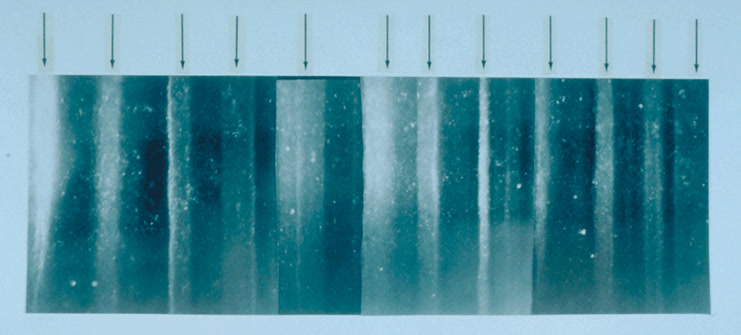
\includegraphics[width=0.78\linewidth]{images/book1/g9-gisp2-layers.jpg}

{\small A section of ice core \qty{19}{cm} long, drilled at a depth of
\qty{1855}{m} in the Greenland \omterm{def:g8:ice-on-earth:ice-sheet}{ice sheet} and lit from below. The arrows
point to the lighter summer layers, between darker winter layers: eleven
years of \omterm{def:g4:clouds-rain-snow:precipitation}{snow}. NOAA Paleoclimatology (public domain, via Wikimedia
Commons).}
% ledger: commons:gisp2-layers
\label{fig:g9:climate-past-and-present:ice-core}
\end{omfigure}

An ice core keeps two records of the past. The \omterm{def:g4:clouds-rain-snow:precipitation}{snow} itself tells how cold
the air was when it fell: the colder the air, the smaller the share of the
heavier forms of hydrogen and oxygen in the \omterm{def:g4:clouds-rain-snow:precipitation}{snow}. And as \omterm{def:g4:clouds-rain-snow:precipitation}{snow} is pressed
into ice, the spaces between the grains close up, trapping tiny bubbles of
the air of the time. Scientists release this ancient air in the
laboratory and measure its carbon dioxide.
% ledger: eo:ice-core

\begin{omfigure}
\begin{tikzpicture}
\begin{axis}[name=temp, omrecord, omage, width=13cm, height=3.9cm, xmin=0, xmax=800,
  xtick={0,100,...,800}, xticklabels={}, ylabel={temperature\\ change ($^\circ$C)},
  ylabel style={align=center}, ymin=-11, ymax=5, ytick={-10,-5,0,5}]
  \addplot[omWarm, line width=0.7pt] table[x=age_kyr, y=temp_C] {figdata/out/grade-9-climate_records-edc.dat};
\end{axis}
\begin{axis}[at={(temp.south west)}, anchor=north west, yshift=-0.3cm, omrecord, omage,
  width=13cm, height=3.9cm, xmin=0, xmax=800, xtick={0,100,...,800},
  xlabel={thousands of years before today}, ylabel={carbon dioxide\\ (ppm)},
  ylabel style={align=center}, ymin=160, ymax=320, ytick={180,220,260,300}]
  \addplot[black, line width=0.7pt] table[x=age_kyr, y=co2_ppm] {figdata/out/grade-9-climate_records-icecore.dat};
\end{axis}
\end{tikzpicture}

{\small Eight hundred thousand years read in the ice of Antarctica. Top:
the change in air temperature at Dome~C, compared with the average of the
last thousand years (EPICA Dome~C ice core, J.~Jouzel and others, 2007).
Bottom: the carbon dioxide of the air trapped in the ice, in parts per
million (B.~Bereiter and others, 2015). Both averaged over steps of
\num{2000} years; time runs from the left (oldest) to the right (today).}
% ledger: data:edc-jouzel, data:co2-bereiter (figdata/grade-9/climate_records.py)
\label{fig:g9:climate-past-and-present:icecore}
\end{omfigure}

The two curves tell the same story. Again and again, long cold times, the
\omterm{def:g8:ice-on-earth:ice-age}{ice ages}, gave way to shorter warm times, then the cold came back. At the
coldest, the air over Antarctica was about \qty{9}{\degreeCelsius} colder
than in the last thousand years; in the warmest times it was a few
degrees warmer. And the carbon dioxide rose and fell with the temperature,
between about \qty{175}{ppm} in the cold times and about \qty{300}{ppm}
in the warm ones. We live in one of the warm times, which began as the
last \omterm{def:g8:ice-on-earth:ice-age}{ice age} ended.
% ledger: data:edc-jouzel, data:co2-bereiter (figdata/grade-9/climate_records.py: edc min -9.7, max +3.6; CO2 174 to 299 ppm)

\begin{method}[Reading two records side by side]
\begin{enumerate}
  \item Check that the two records share the same time axis, and which
        way time runs.
  \item Pick a date on the time axis and read each record at that date.
  \item Look for peaks and troughs: do they come at the same times in both
        records?
  \item Say what moves together, without deciding yet which change caused
        the other.
\end{enumerate}
\end{method}

\begin{example}[The last ice age in the ice core]
At \num{20000} years before today (the 20 on the time axis), the
temperature curve is at about \qty{-9}{\degreeCelsius} and the carbon
dioxide at about \qty{190}{ppm}. In the last thousand years, the
temperature curve is close to 0 and the carbon dioxide close to
\qty{280}{ppm}. So, at the coldest of the last \omterm{def:g8:ice-on-earth:ice-age}{ice age}, the air over
Antarctica was about \qty{9}{\degreeCelsius} colder, and it held about
$280 - 190 = \qty{90}{ppm}$ less carbon dioxide, a third less.
\end{example}
% ledger: data:edc-jouzel, data:co2-bereiter (figdata/grade-9/climate_records.py: 19-21 kyr bins -9.4, 190 ppm; 1 kyr bin 278)

Further back still, the Earth knew \omterm{def:g5:weather-and-climate:climate}{climates} much warmer than any of the
last 800\,000 years. The scientific assessments estimate that the last
time the Earth's surface stayed \qty{2.5}{\degreeCelsius} or more above
its level of the late 19th century was over three million years ago.
% ledger: ipcc:3myr

\section{The records of today}

Since the late 19th century, the temperature has been measured every day
at thousands of \omterm{def:g4:clouds-rain-snow:weather-station}{weather stations} on land and at \omterm{def:g2:water-on-earth:ocean}{sea}, with thermometers
kept in the shade. To follow the whole planet, scientists do not average
the temperatures themselves, which depend on where each station is, but
how much each one differs from its own usual value.
% ledger: giss:method

\begin{definition}[Temperature anomaly]\label{def:g9:climate-past-and-present:anomaly}
A \emph{temperature anomaly}\index{temperature anomaly} is the difference
between a temperature and its average over a chosen reference period. It
is positive when it is warmer than that average, negative when it is
colder.
\end{definition}

\begin{omfigure}
\begin{minipage}[c]{0.44\linewidth}\centering
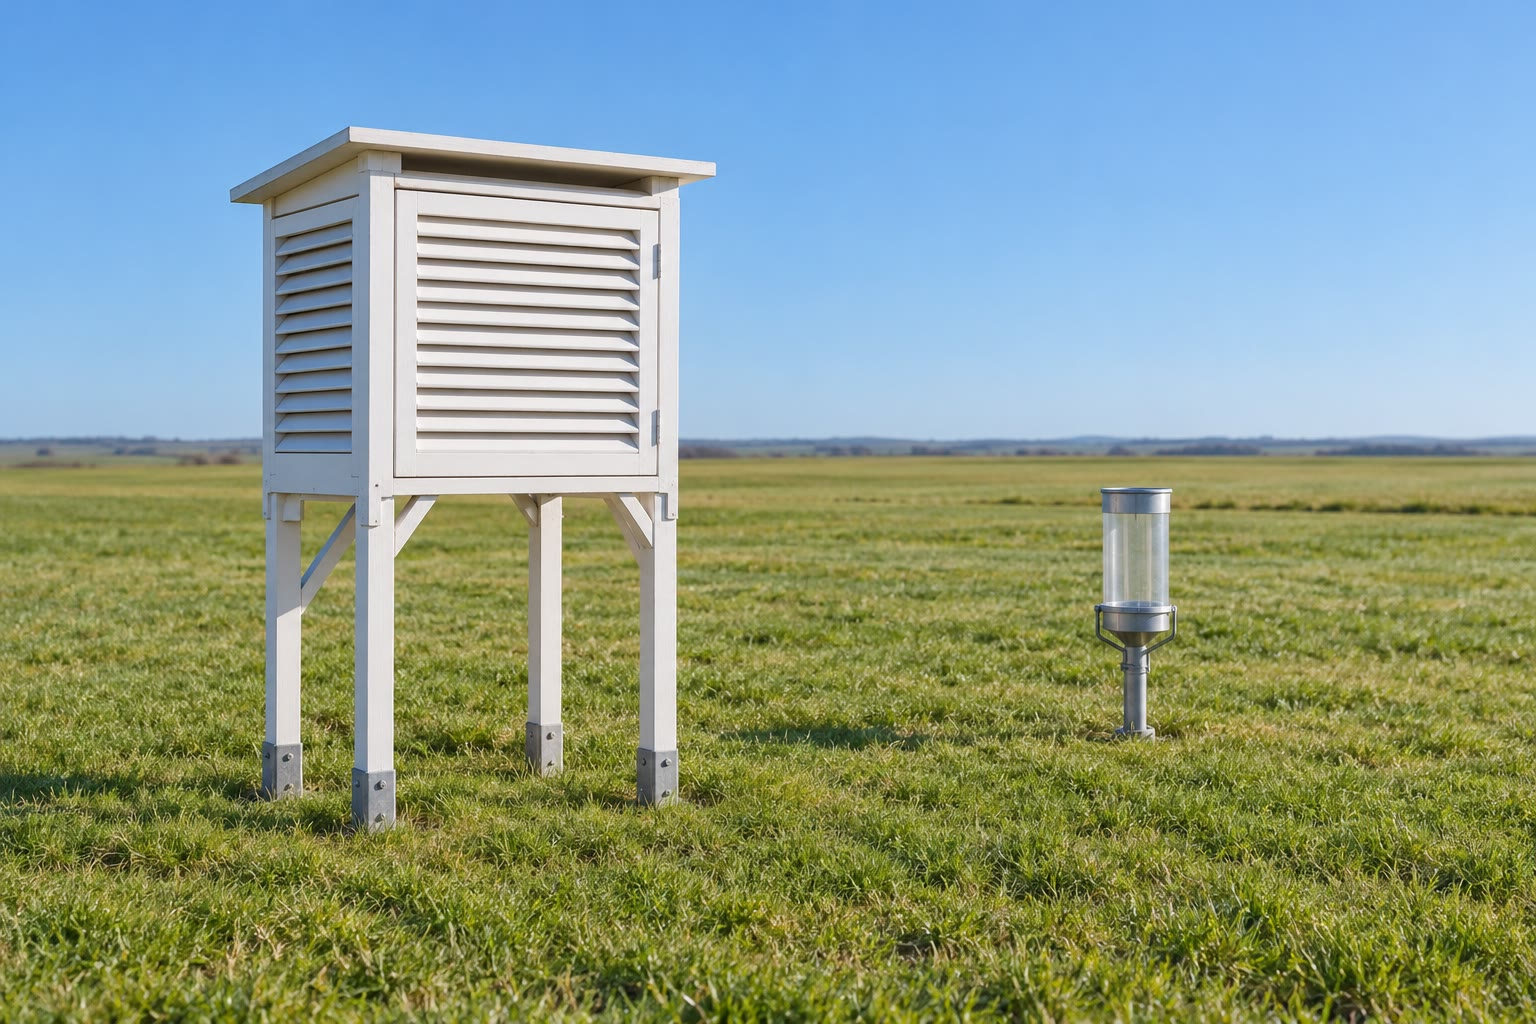
\includegraphics[width=\linewidth]{images/book1/ai/g9-weather-screen.jpg}
\end{minipage}\hfill
\begin{minipage}[c]{0.52\linewidth}\raggedright
{\small A \omterm{def:g4:clouds-rain-snow:weather-station}{weather station}: the white box on legs, with slatted sides,
keeps the thermometers in the shade while the air flows through it; on
the right, a \omterm{def:g4:clouds-rain-snow:rain-gauge}{rain gauge} (AI-generated illustration of a generic scene).}
\end{minipage}
\label{fig:g9:climate-past-and-present:screen}
\end{omfigure}

The NASA record of the global temperature, for instance, gives each
year's anomaly compared with the average of 1951--1980, from land
stations and from measurements of the \omterm{def:g2:water-on-earth:ocean}{sea} surface. Averaged decade by
decade, it shows a clear rise.
% ledger: giss:method, data:gistemp

\begin{omfigure}
\begin{tikzpicture}
\begin{axis}[omrecord, ybar, width=13cm, height=5.6cm, bar width=9pt,
  ymin=-0.45, ymax=1.2, ytick={-0.4,0,0.4,0.8,1.2},
  xtick=data, xticklabels from table={figdata/out/grade-9-climate_records-decades.dat}{label},
  x tick label style={rotate=60, anchor=east, font=\scriptsize},
  ylabel={temperature anomaly ($^\circ$C)}, xmajorgrids=false]
  \addplot[fill=omWarm!70, draw=black!50] table[x expr=\coordindex, y=mean_C]
    {figdata/out/grade-9-climate_records-decades.dat};
\end{axis}
\end{tikzpicture}

{\small The global surface temperature, decade by decade since the 1880s,
as an anomaly compared with the 1951--1980 average; the last bar covers
the six years 2020--2025. Data: NASA GISTEMP version~4.}
% ledger: data:gistemp (figdata/grade-9/climate_records.py)
\label{fig:g9:climate-past-and-present:decades}
\end{omfigure}

\begin{definition}[Global warming]\label{def:g9:climate-past-and-present:global-warming}
\emph{Global warming}\index{global warming} is the rise of the average
temperature of the Earth's surface, as a whole, since the second half of
the 19th century.
\end{definition}

Year by year, the record goes up and down: one year can be cooler than the
one before, because the \omterm{def:g1:watching-the-weather:weather}{weather} of a whole year, over \omterm{def:g2:water-on-earth:ocean}{oceans} and
\omterm{def:g3:continents-and-oceans:continent}{continents}, varies too. To measure a warming, scientists therefore compare
averages over many years, never two single years.

\begin{omfigure}
\begin{tikzpicture}
\begin{axis}[omrecord, width=13cm, height=5.4cm, xmin=1875, xmax=2030, ymin=-0.6, ymax=1.4,
  xtick={1880,1900,...,2020}, x tick label style={/pgf/number format/1000 sep={}},
  xlabel={year}, ylabel={temperature anomaly ($^\circ$C)},
  legend style={at={(0.2,0.97)}, anchor=north west, draw=none, fill=white, font=\footnotesize}]
  \fill[omWarm!10] (axis cs:1880,-0.6) rectangle (axis cs:1899,1.4);
  \fill[omWarm!10] (axis cs:2015,-0.6) rectangle (axis cs:2024,1.4);
  \addplot[black!70, mark=*, mark size=0.9pt, line width=0.4pt]
    table[x=year, y=anomaly_C] {figdata/out/grade-9-climate_records-annual.dat};
  \addlegendentry{each year}
  \addplot[omWarm, line width=2pt] table[x=year, y=mean_C] {figdata/out/grade-9-climate_records-periods.dat};
  \addlegendentry{mean of a period}
  \draw[dashed, black!50] (axis cs:1875,0) -- (axis cs:2030,0);
  \node[font=\scriptsize, fill=white, inner sep=1pt] at (axis cs:1889.5,0.45) {1880--1899};
  \node[font=\scriptsize, fill=white, inner sep=1pt] at (axis cs:2019.5,0.3) {2015--2024};
\end{axis}
\end{tikzpicture}

{\small The global \omterm{def:g9:climate-past-and-present:anomaly}{temperature anomaly} of every year from 1880 to 2025
(compared with the 1951--1980 average, dashed line), with the means of two
periods of the problem of this chapter: 1880--1899 and 2015--2024. Data:
NASA GISTEMP version~4.}
% ledger: data:gistemp (figdata/grade-9/climate_records.py)
\label{fig:g9:climate-past-and-present:annual}
\end{omfigure}

\begin{method}[Measuring a warming between two periods]
\begin{enumerate}
  \item Choose two periods of at least ten years each, one early and one
        late, so that the ups and downs of single years cancel out.
  \item Average the yearly anomalies of each period.
  \item Subtract the early mean from the late one: the result is the
        warming between the two periods, in degrees.
  \item Say which record and which periods you used: another record, or
        other periods, give a slightly different number.
\end{enumerate}
\end{method}

\begin{example}[The warming since the 1970s]
In the NASA record, the anomalies of the ten years 1970--1979 average
\qty{0.03}{\degreeCelsius}, and those of 2010--2019 average
\qty{0.80}{\degreeCelsius}. The warming between these two decades is
$0.80 - 0.03 = \qty{0.77}{\degreeCelsius}$, in forty years: about
\qty{0.19}{\degreeCelsius} per decade. Single years, also forty years
apart, would give very different answers: 1976 ($-0.10$) against 2016
(1.01) gives \qty{1.11}{\degreeCelsius}, but 1979 (0.16) against 2011
(0.61) gives only \qty{0.45}{\degreeCelsius}.
\end{example}
% ledger: data:gistemp (figdata/grade-9/climate_records.py: decade_1970s 0.03, decade_2010s 0.80; annual 1976 -0.10, 2016 1.01, 1979 0.16, 2011 0.61)

The carbon dioxide of the air has been measured directly since March 1958,
at an observatory about \qty{3400}{m} up the slopes of the Mauna Loa
\omterm{def:g4:volcanoes-earthquakes-first-look:volcano}{volcano}, in Hawaii. In 1959, its yearly average was \qty{316}{ppm}; by
2025, it had reached \qty{427}{ppm}, far above the \qty{300}{ppm} that it
never exceeded in 800\,000 years of ice. It rises faster and faster: by
less than \qty{1}{ppm} a year in the 1960s, by more than \qty{2.5}{ppm} a
year in the last ten years.
% ledger: gml:keeling, data:co2-mlo, data:co2-bereiter (figdata/grade-9/climate_records.py: 315.98, 427.35, 0.86 and 2.63 ppm/yr; ice core max 298.6)

\begin{omfigure}
\begin{tikzpicture}
\begin{axis}[omrecord, width=12cm, height=5cm, xmin=1955, xmax=2030,
  ymin=290, ymax=440, ytick={300,350,400}, xtick={1960,1970,...,2020},
  x tick label style={/pgf/number format/1000 sep={}},
  xlabel={year}, ylabel={carbon dioxide (ppm)}]
  \addplot[black, line width=0.9pt, mark=*, mark size=0.8pt] table[x=year, y=co2_ppm] {figdata/out/grade-9-climate_records-co2.dat};
  \draw[dashed, omWarm] (axis cs:1955,300) -- (axis cs:2030,300);
\end{axis}
\end{tikzpicture}

{\small The carbon dioxide of the air at Mauna Loa, Hawaii, yearly means
1959--2025 (NOAA Global Monitoring Laboratory and Scripps Institution of
Oceanography). The dashed line at \qty{300}{ppm} is about the highest
level found in 800\,000 years of Antarctic ice.}
% ledger: data:co2-mlo, data:co2-bereiter (figdata/grade-9/climate_records.py)
\label{fig:g9:climate-past-and-present:co2}
\end{omfigure}

\begin{dated}{2025}
The yearly average carbon dioxide at Mauna Loa was \qty{427.35}{ppm} in
2025. In the NASA record, the warmest year since 1880 was 2024, with an
anomaly of \qty{1.28}{\degreeCelsius} compared with 1951--1980.
% ledger: data:co2-mlo, data:gistemp (figdata/grade-9/climate_records.py)
\end{dated}

The \omterm{def:g2:water-on-earth:ocean}{sea} is rising too. Since 1993, satellites have measured the height
of the \omterm{def:g2:water-on-earth:ocean}{sea} surface all over the \omterm{def:g3:continents-and-oceans:globe}{globe}: the trend line of their record
rises by about \qty{3.2}{mm} a year, about \qty{10}{cm} in thirty years.
Two things raise the \omterm{def:g2:water-on-earth:ocean}{sea}: water that warms expands, and melting ice on
land adds water to the \omterm{def:g2:water-on-earth:ocean}{ocean}. And the ice is shrinking: \omterm{def:g1:landscapes-around-us:landform}{mountain} \omterm{def:g8:ice-on-earth:glacier}{glaciers}
almost everywhere are retreating, and the Arctic's summer \omterm{def:g8:ice-on-earth:sea-ice}{sea ice} has lost
almost half of its extent since 1979 (\cref{ch:g8:ice-on-earth}).
% ledger: data:gmsl-lsa (figdata/grade-9/climate_records.py: 3.18 mm/yr; 101 mm 1993-2024), ipcc:b1-ice, nsidc:ice-shelves, data:b1-nsidc-sea-ice

\begin{omfigure}
\begin{tikzpicture}
\begin{axis}[omrecord, width=12cm, height=4.8cm, xmin=1992, xmax=2026,
  ymin=-30, ymax=100, xtick={1995,2000,...,2025},
  x tick label style={/pgf/number format/1000 sep={}},
  xlabel={year}, ylabel={sea level (mm)},
  legend style={at={(0.02,0.97)}, anchor=north west, draw=none, fill=white, font=\footnotesize}]
  \addplot[omCold, mark=*, mark size=1.1pt, line width=0.6pt] table[x=year, y=gmsl_mm] {figdata/out/grade-9-climate_records-sea.dat};
  \addlegendentry{yearly mean}
  \addplot[omWarm, dashed, line width=0.9pt] table[x=year, y=gmsl_mm] {figdata/out/grade-9-climate_records-sea-trend.dat};
  \addlegendentry{trend line}
\end{axis}
\end{tikzpicture}

{\small The global mean \omterm{def:g4:world-physical-map:altitude}{sea level} measured by satellites, yearly means
1993--2024, compared with a reference level, and its trend line (NOAA
Laboratory for Satellite Altimetry).}
% ledger: data:gmsl-lsa (figdata/grade-9/climate_records.py)
\label{fig:g9:climate-past-and-present:sea}
\end{omfigure}

\section{Climate change and its causes}

\begin{definition}[Climate change]\label{def:g9:climate-past-and-present:climate-change}
\emph{Climate change}\index{climate change} is a change in the \omterm{def:g5:weather-and-climate:climate}{climate}
of the Earth, or of a region, that lasts for decades or longer: a change
of its average temperature, \omterm{def:g4:clouds-rain-snow:precipitation}{rain}, winds or ice, not just one unusual
season.
\end{definition}

The \omterm{def:g5:weather-and-climate:climate}{climate} has always changed, as the ice cores show. What is new is
the speed of today's change, and its cause. Scientists from all over the
world regularly assess what has been published on the \omterm{def:g5:weather-and-climate:climate}{climate}, in the
reports of the Intergovernmental Panel on Climate Change (IPCC). The
reports weigh how sure each statement is, with words chosen with care.

In these reports, each of the words below has a fixed meaning: the chances
in 100 that the statement is true.

\begin{center}
{\small
\begin{tabular}{|l|c||l|c|}
\hline
\emph{virtually certain} & 99 to 100 & \emph{likely} & 66 to 100 \\
\emph{extremely likely} & 95 to 100 & \emph{about as likely as not} & 33 to 66 \\
\emph{very likely} & 90 to 100 & \emph{unlikely} & 0 to 33 \\
\hline
\end{tabular}}
\end{center}
% ledger: ipcc:likelihood

\noindent A few statements carry none of these words: they are given as
facts, such as ``it is \emph{unequivocal}''. When you read a news story
about the \omterm{def:g5:weather-and-climate:climate}{climate}, look for these words, and notice which ones the story
keeps and which it drops.
% ledger: ipcc:unequivocal

The assessment published in 2021 states the following.
\begin{itemize}
  \item It is \emph{unequivocal} that human influence has warmed the
        atmosphere, the \omterm{def:g2:water-on-earth:ocean}{ocean} and the land.
  \item The global surface temperature of 2011--2020 was about
        \qty{1.1}{\degreeCelsius} higher than in 1850--1900, and each of
        the last four decades was warmer than any decade before it since
        1850.
  \item The \emph{likely} human-caused warming from 1850--1900 to
        2010--2019 is 0.8 to \qty{1.3}{\degreeCelsius}, with a best
        estimate of \qty{1.07}{\degreeCelsius}: about the whole of the
        observed warming. Natural causes together changed
        the temperature by only $-0.1$ to $+\qty{0.1}{\degreeCelsius}$.
  \item The carbon dioxide of the air in 2019 was higher than at any time
        in at least two million years (\emph{high confidence}); it had
        risen by 47~\% since 1750.
  \item Human influence is \emph{very likely} the main cause of the
        retreat of \omterm{def:g8:ice-on-earth:glacier}{glaciers} since the 1990s and of the shrinking of the
        Arctic \omterm{def:g8:ice-on-earth:sea-ice}{sea ice}; and \emph{very likely} the main cause of the rise
        of the \omterm{def:g2:water-on-earth:ocean}{sea} since at least 1971.
\end{itemize}
% ledger: ipcc:unequivocal, ipcc:gsat-2011-2020, ipcc:decades, ipcc:attribution, ipcc:co2-2myr, ipcc:b1-ice, ipcc:sea-level-obs

\begin{history}[Charles David Keeling's curve]
In March 1958, a young chemist of the Scripps Institution of
Oceanography, Charles David Keeling, began measuring the carbon dioxide
of the air on Mauna Loa, high above the \omterm{def:g2:water-on-earth:ocean}{sea} and far from any town. His
measurements have gone on ever since: they are the longest record of
carbon dioxide measured directly in the air, and the curve they draw,
rising year after year, carries his name, the \emph{Keeling curve}.
% ledger: gml:keeling
\end{history}

Why does the warming follow the carbon dioxide? Burning coal, oil and gas
releases carbon dioxide; more carbon dioxide in the air means that more
of the infrared light given off by the surface is absorbed and sent back
down, and the surface warms. Water vapour, methane and the other
greenhouse gases add to the effect. The past and the present agree: in the
ice cores as in today's records, the Earth's temperature and its carbon
dioxide rise and fall together.
% ledger: ipcc:attribution, ipcc:co2-2myr

\section{Exercises}

\begin{exercise}[$\star$]\label{exo:g9:climate-past-and-present:1}
% ledger: earth:Tbb, earth:Tsurf
(a) What would the average temperature of the Earth's surface be without
the greenhouse effect? (b) What is it with it? (c) By how many degrees
does the greenhouse effect warm the surface? (d) Name two greenhouse
gases.
\end{exercise}

\begin{exercise}[$\star$]\label{exo:g9:climate-past-and-present:2}
\omterm{def:g1:watching-the-weather:weather}{Weather} or \omterm{def:g5:weather-and-climate:climate}{climate}? (a) It rained all day yesterday. (b) Summers in this
region are hot and dry. (c) The 2010s were warmer than the 1980s
worldwide. (d) Next week will be cold.
\end{exercise}

\begin{exercise}[$\star$]\label{exo:g9:climate-past-and-present:3}
% ledger: commons:gisp2-layers
Look at the photograph of the ice core section. (a) How long is the
section, and how many years of \omterm{def:g4:clouds-rain-snow:precipitation}{snow} does it hold? (b) Find the average
thickness of one year's layer, in centimetres. (c) Why is the deepest
ice of an \omterm{def:g8:ice-on-earth:ice-sheet}{ice sheet} the oldest?
\end{exercise}

\begin{exercise}[$\star$]\label{exo:g9:climate-past-and-present:4}
A town's average July temperature over 1991--2020 is
\qty{21.0}{\degreeCelsius}. Give the \omterm{def:g9:climate-past-and-present:anomaly}{temperature anomaly} of a July
averaging (a) \qty{22.4}{\degreeCelsius}; (b) \qty{20.3}{\degreeCelsius};
(c) \qty{21.0}{\degreeCelsius}. (d) What does a negative anomaly mean?
\end{exercise}

\begin{exercise}[$\star\star$]\label{exo:g9:climate-past-and-present:5}
% ledger: data:gistemp (figdata/grade-9/climate_records.py)
Use the bar chart of the decades. (a) Which decades were colder than the
1951--1980 average? (b) Read the anomaly of the 1980s and of the 2010s.
(c) By how much did the anomaly grow between these two decades? (d) Is
the rise steady from one decade to the next over the whole record?
\end{exercise}

\begin{exercise}[$\star\star$]\label{exo:g9:climate-past-and-present:6}
% ledger: data:co2-mlo (figdata/grade-9/climate_records.py)
At Mauna Loa, the yearly average carbon dioxide was \qty{315.98}{ppm} in
1959, \qty{324.62}{ppm} in 1969, \qty{401.01}{ppm} in 2015 and \qty{427.35}{ppm} in 2025. (a) What was the
average rise per year from 1959 to 1969? (b) From 2015 to 2025? (c) How
many times faster was the rise in the second period? (d) By how many
percent did the carbon dioxide grow from 1959 to 2025?
\end{exercise}

\begin{exercise}[$\star\star$]\label{exo:g9:climate-past-and-present:7}
% ledger: data:edc-jouzel, data:co2-bereiter
Use the 800\,000-year record. (a) Write 800\,000 years in scientific
notation. (b) About how long ago was the last time it was as warm as
today, before our own warm time? (c) What carbon dioxide level did the
air hold at that time? (d) Do the temperature and the carbon dioxide rise
and fall at the same times?
\end{exercise}

\begin{exercise}[$\star\star$]\label{exo:g9:climate-past-and-present:8}
% ledger: data:gmsl-lsa (figdata/grade-9/climate_records.py)
The \omterm{def:g2:water-on-earth:ocean}{sea} rises by about \qty{3.2}{mm} a year. (a) How much is that in 10
years, in centimetres? (b) If it kept this rate, how much would it rise
between 2025 and 2100? (c) Name two reasons why the \omterm{def:g2:water-on-earth:ocean}{sea} rises. (d) Does
the melting of the Arctic \omterm{def:g8:ice-on-earth:sea-ice}{sea ice} raise the \omterm{def:g2:water-on-earth:ocean}{sea}? Explain.
\end{exercise}

\begin{exercise}[$\star\star$]\label{exo:g9:climate-past-and-present:9}
% ledger: ipcc:likelihood
In the IPCC words, how many chances in 100, at least, does each statement
have of being true? (a) ``It is \emph{very likely}\ldots'' (b) ``It is
\emph{likely}\ldots'' (c) ``It is \emph{virtually certain}\ldots'' (d) A
newspaper writes ``scientists are sure that'' about a statement the report
calls \emph{likely}. What is wrong?
\end{exercise}

\begin{exercise}[$\star\star$]\label{exo:g9:climate-past-and-present:10}
A friend says: ``This winter was the coldest in ten years where I live,
so the Earth is not warming.'' Explain, using the words \emph{\omterm{def:g1:watching-the-weather:weather}{weather}},
\emph{\omterm{def:g5:weather-and-climate:climate}{climate}} and \emph{global}, why this argument does not hold.
\end{exercise}

\begin{exercise}[$\star\star\star$]\label{exo:g9:climate-past-and-present:11}
% ledger: data:co2-bereiter, data:co2-mlo, ipcc:co2-2myr, ipcc:erf-2xco2
At the coldest of the last \omterm{def:g8:ice-on-earth:ice-age}{ice age}, about $2 \times 10^4$ years ago, the
air held about \qty{190}{ppm} of carbon dioxide; just before the
industrial era, about \qty{280}{ppm}; in 2025, about \qty{427}{ppm}.
(a) How much did the carbon dioxide rise from the \omterm{def:g8:ice-on-earth:ice-age}{ice age} to the
industrial era, and in how many years? (b) How much did it rise from
the industrial era to 2025? Take 1750 as the start of the industrial era.
(c) Compare the two rises: in size, and in average rate per year, using
scientific notation. (d) What does the IPCC say about the carbon dioxide
level of today compared with the past?
\end{exercise}

\begin{exercise}[$\star\star\star$]\label{exo:g9:climate-past-and-present:12}
% ledger: ipcc:attribution, ipcc:observed-2010-2019
The IPCC assessment gives the observed warming from 1850--1900 to
2010--2019 as about \qty{1.06}{\degreeCelsius}, and the human-caused
warming as \emph{likely} 0.8 to \qty{1.3}{\degreeCelsius} (best estimate
\qty{1.07}{\degreeCelsius}); the natural causes together are given as
$-0.1$ to $+\qty{0.1}{\degreeCelsius}$. (a) Compare the best estimate of
the human-caused warming with the observed warming. (b) Could natural causes
alone explain the observed warming? Explain. (c) What does
\emph{likely} mean in this sentence?
\end{exercise}

\section{Problem: The planet's thermometer}

\begin{problem}[{Weekend problem --- the warming of the Earth is worked out
from the NASA temperature record, then set beside the carbon dioxide and
the sea}]
\label{pb:g9:climate-past-and-present:1}
% ledger: data:gistemp, data:co2-mlo, data:gmsl-lsa, ipcc:gsat-2011-2020 (figdata/grade-9/climate_records.py)
The table gives the global \omterm{def:g9:climate-past-and-present:anomaly}{temperature anomaly} of the NASA record
(compared with the 1951--1980 average) for some groups of years, and other
records of the chapter.

\begin{center}
{\small
\begin{tabular}{|l|c|}
\hline
mean anomaly, 1880--1899 & \qty{-0.22}{\degreeCelsius} \\
mean anomaly, 1951--1980 & \qty{0.00}{\degreeCelsius} \\
mean anomaly, 2015--2024 & \qty{0.98}{\degreeCelsius} \\
carbon dioxide at Mauna Loa, 1959 / 2025 & \qty{316}{ppm} / \qty{427}{ppm} \\
\omterm{def:g4:world-physical-map:altitude}{sea level} trend from satellites, since 1993 & \qty{3.2}{mm} per year \\
\hline
\end{tabular}}
\end{center}

\noindent\textbf{Part I --- The decades.}\par\nopagebreak
\begin{enumerate}[beginpenalty=10000]
  \item Why is the anomaly of 1951--1980 exactly zero?
  \item Was 1880--1899 warmer or colder than 1951--1980? By how much?
  \item Was 2015--2024 warmer or colder than 1951--1980? By how much?
  \item Compute the warming of 2015--2024 compared with 1880--1899.
\end{enumerate}

\noindent\textbf{Part II --- The carbon dioxide.}\par\nopagebreak
\begin{enumerate}[resume, beginpenalty=10000]
  \item By how many ppm did the carbon dioxide rise between 1959 and 2025?
  \item By what percentage of its 1959 value?
  \item In the ice cores, the carbon dioxide never went above about
        \qty{300}{ppm} in 800\,000 years. By how much does the 2025 value
        exceed it?
  \item Explain in two sentences how more carbon dioxide in the air
        warms the surface.
\end{enumerate}

\noindent\textbf{Part III --- The sea.}\par\nopagebreak
\begin{enumerate}[resume, beginpenalty=10000]
  \item How much has the \omterm{def:g2:water-on-earth:ocean}{sea} risen from 1993 to 2025 at the rate of the
        table, in centimetres?
  \item Name the two causes of this rise.
  \item The IPCC gives the warming of 2011--2020 compared with 1850--1900
        as about \qty{1.09}{\degreeCelsius}. Is your answer to question~4
        of the same size? Give one reason why the two numbers differ a
        little.
  \item Write the sentence a science journalist could print: ``Since the
        end of the 19th century, the Earth's surface has warmed by
        about \ldots''
\end{enumerate}
\end{problem}
